% ===== 原文 pp.33--41（PDF p.43--51）：第 4 章 拓扑场论、范畴与 2-范畴 =====
% ===== 本文件 ch04-02.tex：印刷 pp.37--41（PDF p.47--51） =====

% [原文 p.37]
\begin{figure}[htbp]
\centering
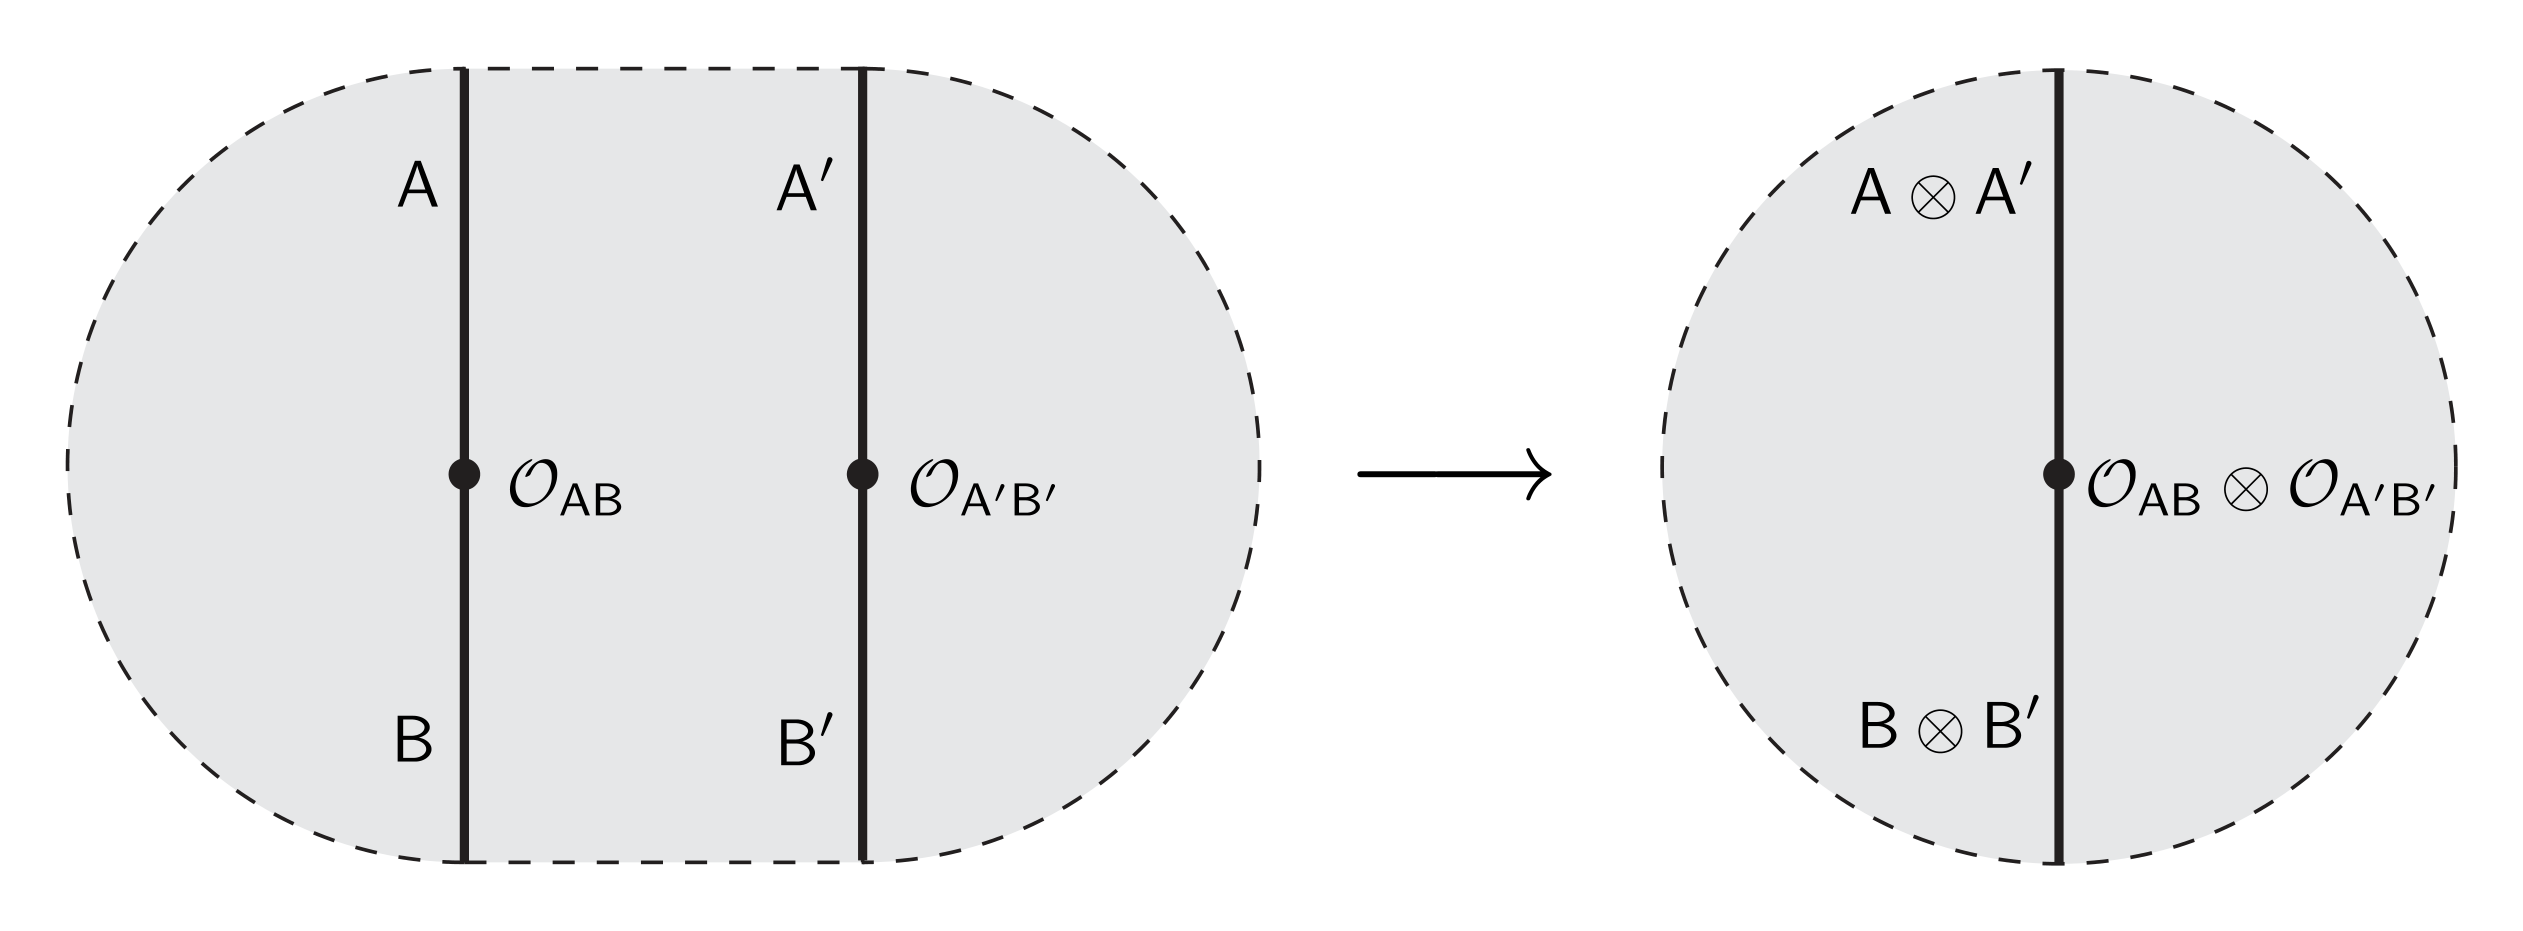
\includegraphics[width=0.85\textwidth]{fig45.png}
\figtitle{4.5}{2d TFT 的 2-范畴中 2-态射的复合，通过融合它们所插入其上的壁来实现。相应的运算记作 $\otimes$。}
\end{figure}

\begin{figure}[htbp]
\centering
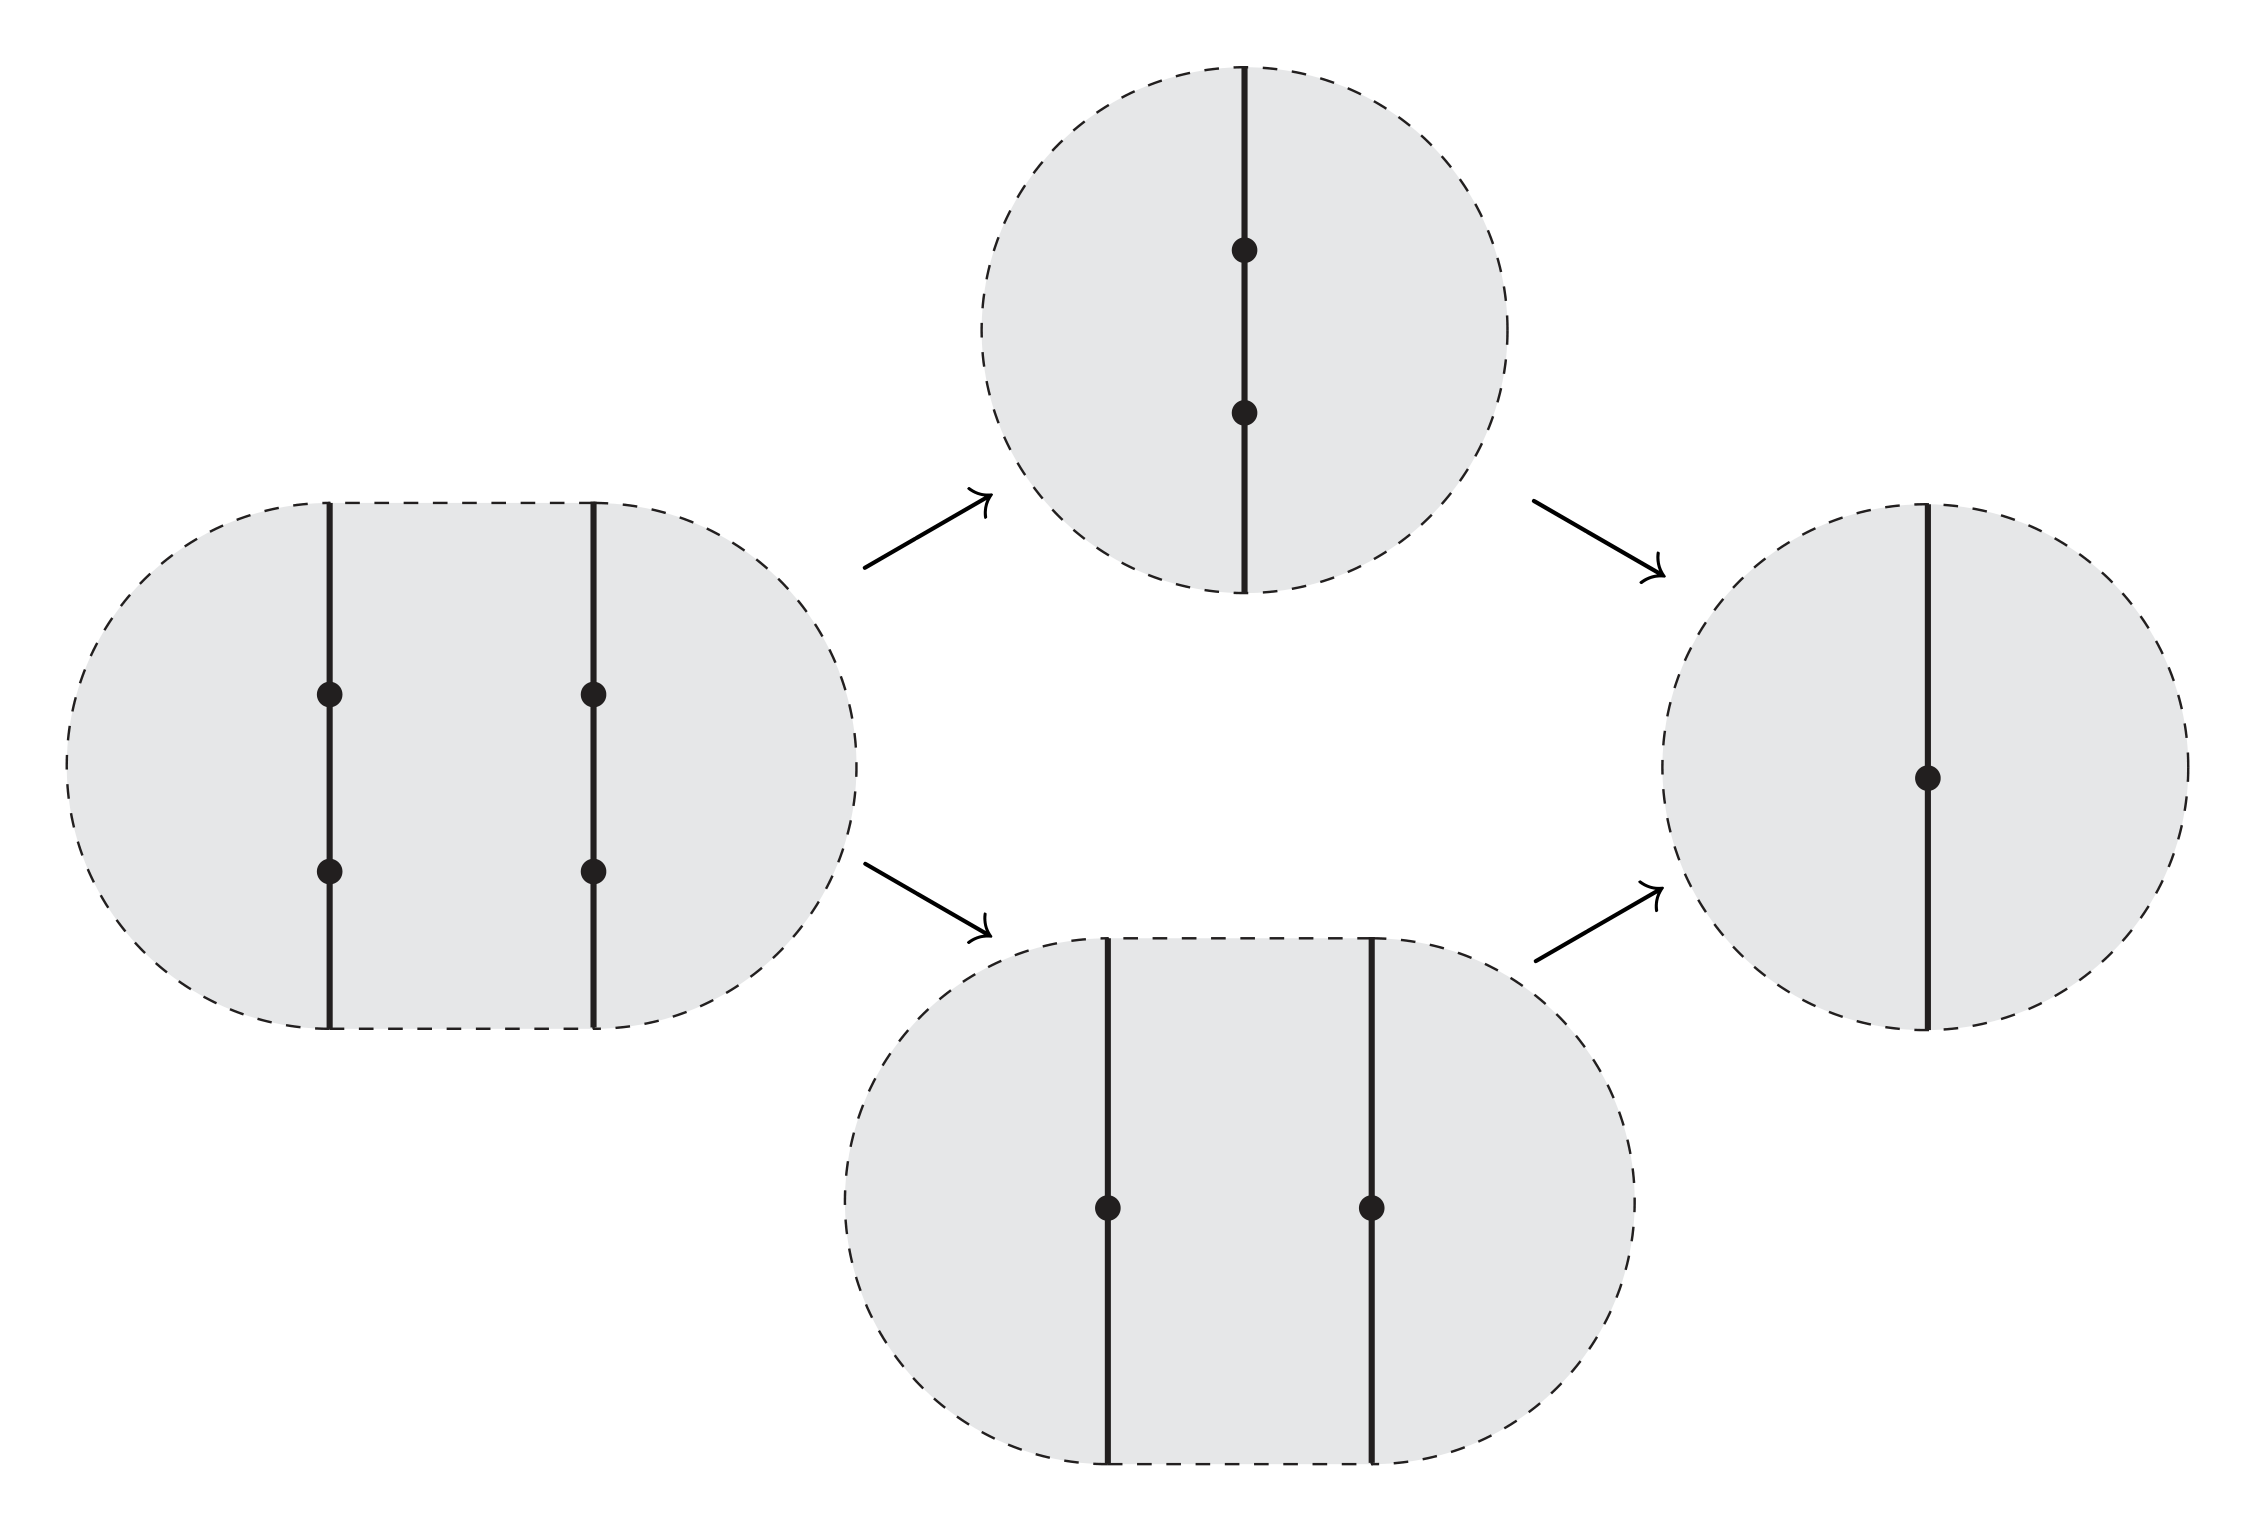
\includegraphics[width=0.5\textwidth]{fig46.png}
\figtitle{4.6}{插在壁上的局部算子既可以看作 2d TFT 范畴的 2-态射，此时复合对应于“水平”融合；也可以看作边界条件范畴的态射，此时复合对应于“竖直”融合。这两种运算相互交换。}
\end{figure}

% [Tutor Note: 图 4.6 的原文图注写作 “2-morphisms of the \emph{category} of 2d TFTs”，按上下文（对照图 4.5 的 “of the 2-category of 2d TFTs”）应为 “2-category”，此处疑为原文笔误。译注本的图注按正确含义译为“2d TFT 范畴的 2-态射”，与图 4.5 的措辞一致。]

% [原文 p.38]
$\mathbb{V}_{\mathbb{X}\mathbb{X}}$ 的对象：
\[
    (\mathsf{A},\mathsf{B})\mapsto \mathsf{A}\otimes\mathsf{B}\in\Ob(\mathbb{V}_{\mathbb{X}\mathbb{X}})
\]

以及态射
\[
    \Mor(\mathsf{A},\mathsf{B})\otimes\Mor(\mathsf{C},\mathsf{D})\to\Mor(\mathsf{A}\otimes\mathsf{C},\mathsf{B}\otimes\mathsf{D}).
\]

这种张量一般不必交换。带有这种额外“张量”结构的范畴称为幺半范畴（monoidal category）。由上面应当清楚：幺半范畴与只有一个对象的 2-范畴是同一回事。

% [Tutor Note: p.38 “同一回事”应理解为（弱）等价：只有一个对象的双范畴与幺半范畴等价，结合子（associator）对应 2-态射层面的结合约束。核对方法：把单对象 2-范畴的 2-态射取成向量空间、1-态射取成对象，则张量积的结合子与幺半范畴的 Mac Lane 融贯条件一一对应；若要求严格相等则得严格幺半范畴。]

在给定 2d TFT 的所有缺陷线中，有一条平凡的缺陷线 $\mathbf{1}$，它等价于完全没有缺陷。我们可以称它为不可见缺陷线（invisible defect line）。它是缺陷线幺半范畴中的单位对象，其意义是：把它与任何其他缺陷线 $\mathsf{A}$ 融合都还原为 $\mathsf{A}$。平凡缺陷线的自同态（即向量空间 $\Mor(\mathbf{1},\mathbf{1})$ 的元素）等同于体（bulk）中的局部算子。

幺半范畴最简单的例子是向量空间范畴，配以通常的张量积。它可以看成一个平凡 2d TFT（例如靶空间为一点的拓扑 $\sigma$-模型）中缺陷线的 2-范畴。Landau-Ginzburg TFT 中的缺陷线已在 [31, 32] 中研究过。

可以把给定 2d TFT 中的一条缺陷线与任意边界条件融合，得到同一 TFT 中的一个新边界条件。这就定义了缺陷线幺半范畴在膜范畴上的一个“作用”。在数学上，可以用模范畴（module category）的概念来描述它。既然幺半范畴是代数这一概念的范畴化，自然就把幺半范畴上的模范畴定义为代数上模这一概念的范畴化。幺半范畴 $\mathbb{V}$ 上的模范畴 $\mathbb{W}$ 的定义，包含一条用 $\mathbb{V}$ 的对象“乘”$\mathbb{W}$ 的对象的规则：
\[
    (\mathsf{A},\mathsf{C})\mapsto\mathsf{A}\cdot\mathsf{C}\in\Ob(\mathbb{W}),\qquad
    \forall\mathsf{A}\in\Ob(\mathbb{W}),\ \forall\mathsf{C}\in\Ob(\mathbb{V}),
\]
以及一条乘态射的规则，即一个映射
\[
    \Mor_{\mathbb{W}}(\mathsf{A},\mathsf{B})\otimes\Mor_{\mathbb{V}}(\mathsf{C},\mathsf{D})\to
    \Mor_{\mathbb{W}}(\mathsf{A}\cdot\mathsf{C},\mathsf{B}\cdot\mathsf{D}).
\]

后一条规则编码了这样的事实：我们可以把一个两条缺陷线的交接点与一个两个边界条件的交接点融合起来，得到一个新的、两个新边界条件的交接点。

% [Tutor Note: p.38 原文 “a rule for ‘multiplying’ an object \emph{on} $\mathbb{W}$ by an object of $\mathbb{V}$” 中的 “on” 疑为 “of” 之笔误（后文一律作 “an object of $\mathbb{W}$”）。核对：取 $\mathbb{V}=\mathrm{Vect}$、$\mathbb{W}=\mathrm{Vect}$，上述两条规则退化为通常的向量空间张量积，即平凡例子。]

我们在本论文中系统地使用的一个重要想法是：余维 2 缺陷的某些性质可以用维数约化来研究。我们已经见过一个简单的例子：坐在两个边界条件 $\mathsf{A}$ 与 $\mathsf{B}$ 交接处的局部算子所构成的空间，可以看成把 2d TFT 在带边界条件 $\mathsf{A}$ 与 $\mathsf{B}$ 的区间上紧化后得到的 1d 场论（即量子力学）的状态空间。

% [原文 p.39]
另一个例子是体中局部算子所构成的空间。众所周知，它可以等同于把 2d TFT 在圆周上紧化后得到的 1d 场论的状态空间。两种情况下的论证本质上相同。挖去局部算子的管状邻域之后，算子插入被一个新生成的边界取代，该边界的领口邻域在第一种情形下形如 $\R_+\times I$，在第二种情形下形如 $\R_+\times S^1$。然后利用 TFT 中管状邻域的大小无关这一点，就可以把新生成的边界上的任意边界条件当作一个局部算子。

% [Tutor Note: p.39 两种情形可按局部几何核对：体内局部算子在 2d 世界面上的管状邻域 $\cong D^2$，其边界是圆 $S^1$，领口为 $\R_+\times S^1$，故对应“在圆上紧化”；而两段边界交接处的算子，其管状邻域是世界面的半圆盘，边界是区间 $I$（$I$ 的两端落在边界线上，分别带 $\mathsf{A}$ 与 $\mathsf{B}$），领口为 $\R_+\times I$，故对应“在区间上紧化”。两者都归结为 1d 场论的状态空间，这正是作者所说“论证本质上相同”。]

值得注意的是，这种把余维 2 缺陷解释为低维理论的做法会造成“信息丢失”。例如，如果把所涉及的向量空间看作三个 1d 场论的状态空间，我们就无法计算复合 $V_{\mathsf{A}\mathsf{B}}\otimes V_{\mathsf{B}\mathsf{C}}\to V_{\mathsf{A}\mathsf{C}}$。同样，如果把体中局部算子的空间看作一个 1d 场论的状态空间，我们就看不到它上面的交换代数结构。

% [Tutor Note: p.39 “信息丢失”的根源：紧化到一维只保留了 $V_{\mathsf{A}\mathsf{B}}$ 作为向量空间，而复合映射 $V_{\mathsf{A}\mathsf{B}}\otimes V_{\mathsf{B}\mathsf{C}}\to V_{\mathsf{A}\mathsf{C}}$ 来自二维世界面在交接处的融合（图 4.2）；一维理论没有任何运算对应于“把两个插入点并合成一点”，故该映射丢失。同理，体中局部算子空间上的交换代数结构来自世界面上算子的彼此交换，一维状态空间也看不到。]

\section{三维 TFT 与边界条件的 2-范畴}

当我们来到三维时，会发现 3d TFT 中的边界条件同样构成一个 2-范畴。为了看出这一点，先考虑一个平凡的 3d TFT（例如靶空间为一点的 3d 拓扑 $\sigma$-模型）。此时虽然体的内部没有自由度，我们仍可以考虑把任意 2d TFT 放在边界上。于是平凡 3d TFT 的所有边界条件的集合，就是所有 2d TFT 的集合，而后者构成一个 2-范畴。2d TFT 之间的壁此时可以解释为 3d 世界体（worldvolume）的二维边界上的缺陷线。给定 2d TFT 的缺陷线幺半范畴，可以重新解释为某个特定边界条件的边界线算子的幺半范畴。

如果体中的 3d TFT 是非平凡的，我们仍然可以把它与边界上的 2d TFT 耦合。不同的边界条件由边界上 2d TFT 的类型以及它与体中自由度的耦合方式来区分。关于这在 Rozansky-Witten 3d TFT 中如何具体实现，见 [36]。同样可以考虑分隔不同边界条件的边界缺陷线，它们的融合以及边界缺陷线上局部算子的融合，可以用边界条件集合上的 2-范畴结构来描述。如果聚焦于某个特定的边界条件，那么这个边界上缺陷线的集合具有幺半范畴的结构。

仿照二维的做法，我们可以考虑不同 3d TFT 之间的壁，或面算子。任意两个 3d TFT $\mathbb{K}$ 与 $\mathbb{L}$ 之间所有壁的集合具有 2-范畴的结构。看出这一点的一种办法是：把世界体沿缺陷面折叠，把壁重新解释为理论 $\bar{\mathbb{K}}\times\mathbb{L}$ 的一个边界，其中 $\bar{\mathbb{K}}$ 是理论 $\mathbb{K}$ 的宇称反转。

% [原文 p.40]
进而，正如二维那样，我们可以把壁与缺陷线以及其上的局部算子融合起来（图 4.7）。

\begin{figure}[htbp]
\centering
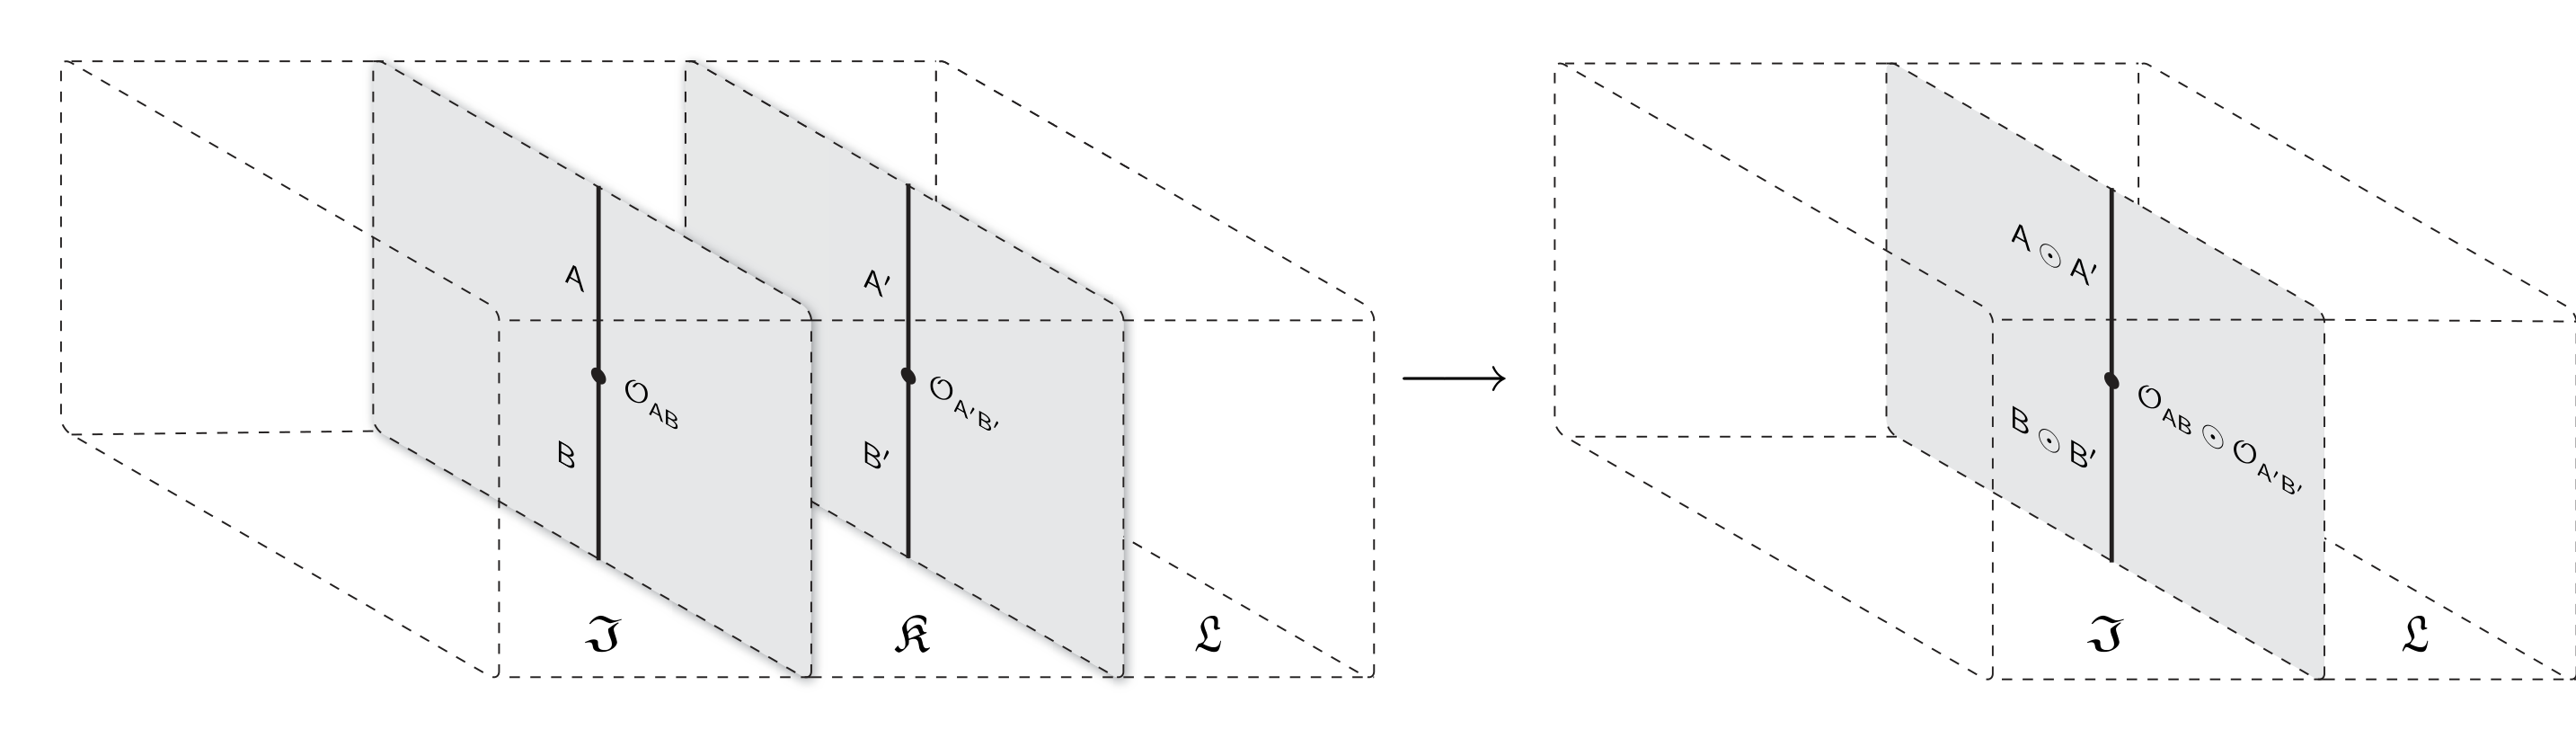
\includegraphics[width=0.85\textwidth]{fig47.png}
\figtitle{4.7}{把缺陷线看作 3d TFT 的 3-范畴的 2-态射、把局部算子看作其 3-态射，就给出它们之间又一种复合运算，我们把它记作 $\odot$。}
\end{figure}

总而言之，可以把这一情形概括为：3d TFT 构成一个 3-范畴。它的对象是 3d TFT，它的态射是 3d TFT 之间的壁，它的 2-态射（态射之间的态射）是壁上的缺陷线，它的 3-态射（2-态射之间的态射）是坐在缺陷线上的局部算子。

% [Tutor Note: p.40 需注意本节两个断言并不矛盾：“$\mathbb{K}$ 与 $\mathbb{L}$ 之间壁的集合构成 2-范畴”讲的是固定两个对象后的 Hom 结构，而“3d TFT 构成 3-范畴”讲的是含对象在内的整体结构；后者把对象忘掉后就退化为前者。核对：把 3-范畴的对象取成一点（即只看一个 3d TFT），其自 Hom 2-范畴恰是“面算子的 2-范畴”，也就是下一段的结论。]

如果把注意力限制在某个特定 3d TFT 中的面算子，我们得到只有一个对象的 3-范畴。等价地说，3d TFT 中面算子的 2-范畴带有额外的结构，使人可以融合对象、态射与 2-态射。换句话说，它是一个幺半 2-范畴。它有一个单位对象（平凡面算子），其自同态可以看成体中的缺陷线。

要确定给定 3d TFT 中体缺陷线的范畴，可以使用维数约化的技巧。为应用它，我们挖去缺陷线的管状邻域，并用其边界上一个合适的边界条件取代这条缺陷线。新生成的边界的领口邻域局部地形如 $S^1\times\R_+\times\R$，其中 $\R_+$ 对应“径向”方向。因此我们可以把缺陷线等同于把 3d TFT 在圆周上紧化所得 2d TFT 中的一个边界条件。这个技巧使人可以通过研究 2d TFT 中的膜范畴来确定体缺陷线的范畴。这样做会丢失一些信息：3d TFT 中体缺陷线的范畴实际上是一个辫幺半范畴（即带有拟交换张量积的范畴），而这一结构无法从二维观点看到。

% [Tutor Note: p.40 的 $S^1\times\R_+\times\R$ 可用维数核对：3d 中缺陷线余维 2，管状邻域 $\cong D^2\times\R$（三维），其边界 $\cong S^1\times\R$，故领口为 $S^1\times\R_+\times\R$；其中 $S^1$ 方向就是用来紧化的圆。这与 §4.4 的 4d 情形 $S^1\times\R_+\times\R^2$（$D^2\times\R^2$ 的边界）完全平行。]

类似地，边界缺陷线范畴的研究可以约化为对把 3d TFT 在区间上紧化所得 2d TFT 中膜范畴的研究。如果边界缺陷线分隔两个边界条件 $\mathbb{X}$ 与 $\mathbb{Y}$，那么区间两端的边界条件应当取 $\mathbb{X}$ 与 $\mathbb{Y}$。这个二维观点同样带来信息丢失：例如，它无法计算范畴 $\mathbb{V}_{\mathbb{X}\mathbb{X}}$ 上的幺半结构。

% [原文 p.41]
\section{四维 TFT 与面算子的 2-范畴}

4d TFT 中的边界条件构成一个 3-范畴。例如，如果 4d TFT 是平凡的，其边界条件的 3-范畴就是所有 3d TFT 的 3-范畴。类似地，给定 4d TFT 中的壁（余维 1 缺陷）构成一个幺半 3-范畴。本论文将避免处理如此复杂的结构，而把注意力集中在余维二的缺陷，即 4d TFT 中的面算子。这样的面算子构成一个 2-范畴。看出这一点的一种办法是应用维数约化技巧：挖去面算子的管状邻域，并用新生成的边界上一个合适的边界条件取代该算子。该边界的领口邻域局部地形如 $S^1\times\R_+\times\R^2$，于是我们可以把面算子重新解释为把 4d 理论在圆周上紧化所得 3d TFT 中的一个边界条件。接着就可以援用已知事实：3d TFT 中的边界条件构成一个 2-范畴。

% [Tutor Note: p.41 的 $S^1\times\R_+\times\R^2$ 同样可核对维数：4d 中面算子余维 2，管状邻域 $\cong D^2\times\R^2$，边界 $\cong S^1\times\R^2$，领口 $S^1\times\R_+\times\R^2$。两条独立论证给出同一结论（圆紧化后的 3d 边界条件 = 2-范畴；四维直接的观点 = 缺陷线上的态射与交接点上的 2-态射），可互为自洽检验。]

当然，也可以直接在四维的语言中解释这个 2-范畴结构的含义。面算子的类型可以越过缺陷线而发生跳变，于是可以把面算子上的缺陷线看成 2-范畴中的态射。坐在两条面缺陷线交接点处的局部算子是 2-态射。四维观点还使人清楚看到，面算子的 2-范畴带有丰富的额外结构。首先，可以把面算子与坐在其上的缺陷线、局部算子一起融合。这就在面算子的 2-范畴上给出一条幺半结构。其次，把面算子四处移动一下，就很容易看出融合运算的拟交换性，即我们得到一个辫幺半 2-范畴。\footnote{辫幺半 2-范畴的一种可能的数学定义在 [34] 中给出。不过，4d TFT 中出现的辫幺半结构似乎属于相当特殊的一类。特别地，其中的辫总是可逆的。}

% [Tutor Note: p.41 脚注称 4d TFT 中的辫总是可逆的，理由可这样理解：让一个面算子绕过另一个再绕回来，整段移动是同位（isotopy），因而构成辫的逆；而一般的辫幺半 2-范畴只要求辫为等价，未必可逆。核对：脚注特意强调“4d TFT 中出现的辫幺半结构属于相当特殊的一类”，正是因为它额外具有这一可逆性，故 [34] 的一般定义未必涵盖 4d 情形的全部结构。]

本论文将使用维数约化技巧，在第 6 章研究我们那些扭转 4d TFT 的面算子 2-范畴；我们不会描述这个 2-范畴上的辫幺半结构。
